\documentclass[12pt]{article}
\usepackage[top=1in, bottom=1in, left=1in, right=1in]{geometry}

\usepackage{setspace}
\onehalfspacing

\usepackage{amssymb}
%% The amsthm package provides extended theorem environments
\usepackage{amsthm}
\usepackage{epsfig}
\usepackage{times}
\renewcommand{\ttdefault}{cmtt}
\usepackage{amsmath}
\usepackage{graphicx} % for graphics files
\usepackage{tabu}

% Draw figures yourself
\usepackage{tikz} 

% writing elements
\usepackage{mhchem}

\usepackage{paralist}

% The float package HAS to load before hyperref
\usepackage{float} % for psuedocode formatting
\usepackage{xspace}

% from Denovo Methods Manual
\usepackage{mathrsfs}
\usepackage[mathcal]{euscript}
\usepackage{color}
\usepackage{array}

\usepackage[pdftex]{hyperref}
\usepackage[parfill]{parskip}

% math syntax
\newcommand{\nth}{n\ensuremath{^{\text{th}}} }
\newcommand{\ve}[1]{\ensuremath{\mathbf{#1}}}
\newcommand{\Macro}{\ensuremath{\Sigma}}
\newcommand{\rvec}{\ensuremath{\vec{r}}}
\newcommand{\omvec}{\ensuremath{\hat{\Omega}}}
\newcommand{\vOmega}{\ensuremath{\hat{\Omega}}}
%---------------------------------------------------------------------------
%---------------------------------------------------------------------------
\begin{document}
\begin{center}
{\bf NE 255, Fa16 \\
Solution Approaches\\
September 22, 2016}
\end{center}

\setlength{\unitlength}{1in}
\begin{picture}(6,.1) 
\put(0,0) {\line(1,0){6.25}}         
\end{picture}

Last class we talked about the reactor problem types and physics involved, as well as how that necessarily impacts the solution strategies we use. Today we'll talk about approaches and what kinds of methods we use when. 

%-------------------------------------------------------------
%-------------------------------------------------------------
\subsection*{Computational Methods}
Inside the box of computational methods, we have two main categories: 
\begin{compactitem}
\item \textbf{Deterministic}: discretize all independent variables, obtain a set of coupled, linear, algebraic equations and develop a numerical method to solve them.
\item \textbf{Probabilistic}: follow the history of each relevant particle based on the underlying probabilities for various types of interactions.
\end{compactitem}
%
Everything we've done so far applies to both methods (we've only simplified the equation). Each method has its own benefits and challenges. We'll talk a bit about \textbf{deterministic first}. Here, the discretization methods are a big part of the strategy, followed by parallelization.

The size of the problems (which impacts memory and parallelization performance) is governed by discretization. The quality and behavior of solutions is also governed by discretization. To get more accurate fluxes, typical transport problems today are three-dimensional, have up to thousands $\times$ thousands $\times$ thousands of mesh points, use up to $\sim$150 energy groups, include accurate expansions of scattering terms, and are solved over many directions. 
%
\begin{table}[!h]
\caption{Meaning and Range of Indices Used in Transport Discretization}
\begin{center}
\begin{tabular}{l c c c c c c}
\hline
Variable & Symbol & First & Last & Low & High \\[0.5ex]
\hline
Energy & g & 1 & G & 2 & 100s \\
Solid Angle & a & 1 & n & $S_2$ & $S_{16}$ \\
Space & n/a & n/a & n/a & 1? & 1e9 \\
Legendre moment ($P_{N}$) & $l$ & 0 & N & 0 & 9 \\
%Spherical harmonic moment ($Y$) & m & 0 & $l$ \\
\hline
\end{tabular}
\end{center}
\label{table:index}
\end{table}

E.g.\ In 2012, a Pressurized Water Reactor (PWR)-900 with 44 groups, a 578 $\times$ 578 $\times$ 700 mesh, using $S_{16}$ level-symmetric quadrature, and with $P_{0}$ scattering was solved: 1.7 trillion unknowns.

With \textbf{Monte Carlo}, we sample the physics of every single interaction of every single particle until we have enough samples to assert that something is statistically valid. This requires lots and lots of samples, but is typically fairly easy to parallelize. Monte Carlo requires strategies and rules for sampling the physics--which can be complicated. 
\begin{figure}[h!]
    \begin{center}
    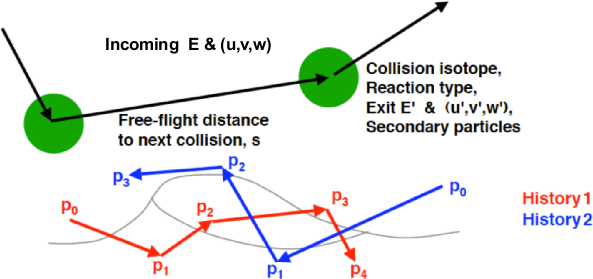
\includegraphics[keepaspectratio, width = 4 in]{MC}
    \end{center}
    \caption{Monte Carlo particle tracking}
    \label{fig:mc}
\end{figure}

\subsubsection*{Diffusion Equation}
Note: in this class we're skipping the diffusion equation. That is what we use in NE155. Just to say a few words:

The diffusion equation removes the angle dependence and gives only $\phi$ as a solution. Nuclear reactions and thus interaction rates only depend on the scalar flux, so maybe that's sufficient.

The diffusion equation is derived by starting with the transport equation and \textbf{integrating over all angles}. In the derivation we make the following assumptions
\begin{compactitem}
\item the scattering term is azimuthally symmetric
\item assume that scattering is at most linearly anisotropic [$P_1$ expansion]
\item assume that the angular flux is at most linearly anisotropic [expand $\psi$ in Legendre polynomials out to $P_1$]
\end{compactitem} 
All of that gives
\begin{equation}
\boxed{\frac{1}{v}\frac{\partial}{\partial t}\phi(\vec{r}, E, t) 
-\nabla \cdot D(\vec{r}, E)\nabla \phi(\vec{r}, E, t) + 
\Sigma_a(\vec{r},E) \phi(\vec{r}, E, t) =
\nu \Sigma_f(\vec{r},E) \phi(\vec{r}, E, t) +
S(\vec{r}, E, t)} \nonumber
\end{equation}
where
\[D = \frac{1}{3\Macro_{tr}} = \frac{1}{3(\Macro_t(\vec{r}) - \Macro_{s1}(\vec{r}))}\:.\] 
is the diffusion coefficient. 

This equation \textit{now includes several assumptions} that are \textbf{valid} when the solution is \textbf{not} near
%
\begin{compactitem}
\item a void, 
\item boundary, 
\item source, 
\item or strong absorber.
\end{compactitem} 
%
While these requirements can be quite restrictive, the diffusion equation has been used frequently for analysis of nuclear systems throughout the history of the nuclear industry.

\subsection*{Comparison}
In order of increasing accuracy\textit{ and} increasing runtime: 
\begin{enumerate}
\item Diffusion Theory
  \begin{compactitem}
  \item discretized and homogenized space
  \item linearly anisotropic direction
  \item discretized energy (few-group)
  \end{compactitem}
\item Deterministic
  \begin{compactitem}
  \item discretized space
  \item discretized direction (discrete ordinates [$S_N$]) or 
        functional expansion of direction (spherical harmonics)
  \item discretized energy (multi-group)
  \end{compactitem}
\item Monte Carlo
  \begin{compactitem}
  \item continuous spatial resolution
  \item continuous direction representation
  \item continuous energy representation
  \end{compactitem}
\end{enumerate}


\begin{center}
\begin{tabu}{| l | X | X |}
  \hline
  & Monte Carlo         & Deterministic \\\hline
    % -----------------------
    Strengths & * General geometry    & * Fast \\
              & * Continuous Energy   & * Global Solution\\
              & * Continuous in Angle & * Solution is of same quality everywhere\\
              & * Inherently 3-D      & * Inputs can be pretty simple \\
              & * Easy to parallelize on CPUs & \\\hline
    % -----------------------
    Weaknesses & * Slow & * Variable discretization governs solution quality \\
               & * Might be memory intensive & * Might be memory intensive \\
               & * Solutions have statistical error & * Solution contains truncation error\\
               & * Local solutions only & * Constrained by what you can mesh \\
               & * Must adequately sample phase space & * Ray Effects \\
               & * Need efficient VR & * Can be complicated to parallelize on CPUs \\
               & * Input can be extremely complicated & \\\hline
\end{tabu}
\end{center}
We tend to think of Monte Carlo as ``benchmark quality" and highly flexible. \\
What is one major hazard of Monte Carlo?\\
What is the biggest challenge of using MC for detailed design?

\end{document}